\pdfoutput=1

\documentclass{l4proj}

%
% put any packages here
%
\usepackage{subcaption}
\usepackage{enumitem}
\usepackage{url}
\usepackage{booktabs}
\usepackage{alltt}
\usepackage{wrapfig}
\usepackage{listings}
\usepackage{color}

\definecolor{dkgreen}{rgb}{0,0.6,0}
\definecolor{gray}{rgb}{0.5,0.5,0.5}
\definecolor{mauve}{rgb}{0.58,0,0.82}
\lstset{frame=tb,
  language=Java,
  aboveskip=3mm,
  belowskip=3mm,
  showstringspaces=false,
  columns=flexible,
  basicstyle={\small\ttfamily},
  numbers=left,
  numberstyle=\color{gray},
  keywordstyle=\color{blue},
  commentstyle=\color{dkgreen},
  stringstyle=\color{mauve},
  breaklines=true,
  breakatwhitespace=true,
  tabsize=4
}

\begin{document}
\title{Animation of the Contextual Analysis and Code Generation Phases of a Compiler}
\author{David Robertson}
\date{January 1, 2000}
\maketitle

\begin{abstract}

\end{abstract}

\educationalconsent
%
%NOTE: if you include the educationalconsent (above) and your project is graded an A then
%      it may be entered in the CS Hall of Fame
%
\tableofcontents
%==============================================================================

\chapter{Introduction}
\pagenumbering{arabic}
With increasing technological advances and furthering levels of software abstraction, some may consider compilation to be a slightly esoteric subject, in that, broad knowledge of compilation theory is typically unnecessary in a modern environment, being required only in a small number of highly specialised industries. Nevertheless, remaining as a cornerstone of a computer science curriculum at many schools and universities is the art of compiler construction, behaviour and optimisation. Why is this?

When questioned on the necessity of teaching compilation, Niklaus Wirth, the creator of the \textit{Pascal} programming language and renowned lecturer of compiler design states, ``\textit{knowledge about system surfaces alone is insufficient in computer science; what is needed is an understanding of contents}'' \cite{WirthTheory}. Wirth's view is one that many share, in the respect that the most successful computer scientists must have more than a superficial understanding of which approaches to follow in a given situation. They must understand how various components interact and why they behave the way they do. To gain a true understanding of the building blocks of computer science is to gain a greater insight into the scientific and mathematical concepts within the field, which provides the most effective means of making informed technological decisions. 

Compilation theory is a foundational component of computer science, upon which a larger syllabus can be developed. To students, the benefits of learning about compilation are perhaps not in its direct application, but in its ability to act as the stepping stone that facilitates a more comprehensive grasp of other concepts; concepts which themselves are grounded in compilation theory.  

\section{Motivation}
Compilation can often be a challenging field to teach effectively. Many elements of compilation involve the generation and traversal of complex, abstract data structures. Abstract, conceptual notions such as these are notoriously difficult both for students to understand and for educators to explain. We desire to find a solution to this problem by creating techniques that provide concrete representations of these types of abstract ideas.

As a common approach to this issue, an educator will attempt to visualise the data structures and the traversals over them. The educator usually does this by creating some sort of ``slideshow'', using an application such as Microsoft PowerPoint. The slides contain a pictorial representation of the data structure in question, and each slide demonstrates a distinct step of the traversal over that data structure. For example, an educator seeking to teach students about a depth-first traversal over a binary tree might design their slideshow similarly to Figure \ref{fig:slideshow}, where we see that each consecutive slide illustrates the next step of the traversal by highlighting the corresponding node.

\begin{figure}
\centering
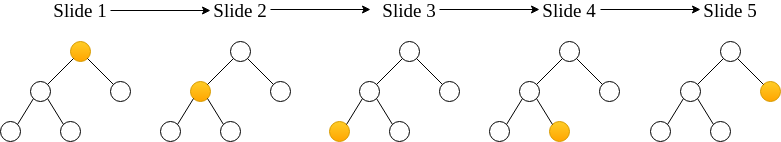
\includegraphics[scale=0.5]{images/slideshow.png}
\caption{A sequence of slides demonstrating a depth-first traversal over a binary tree}
\label{fig:slideshow}	
\end{figure}

Whilst using a slideshow to demonstrate these concepts does provide part of the solution to representing abstract notions, they do have several limitations. Firstly, to create visualisations in this way is an arduous task on behalf of the educator, realistically meaning that the length of the demonstration must remain short. Secondly, there is a limited amount of control over the “playback” of the slides in regards to playing, pausing, rewinding and restarting; which of these functions is possible depends on the choice and availability of slideshow application. Thirdly, and most importantly, the educator is restricted to showing pre-determined examples only. In the case of compilation, not only can the input be completely arbitrary, but the semantics of the compiler varies for each unique construct in the source language. This means pre-determined examples are almost guaranteed to omit certain details, making it difficult for students to achieve a broad and complete understanding.

\section{Aims}
This project aims to alleviate or solve many of the issues currently faced in attempts to create effective visualisations of various compilation concepts. The project will provide a web application in which users will be able to animate the \textit{\textbf{contextual analysis}} and \textit{\textbf{code generation}} phases of the \textit{\textbf{Fun}} compiler. The animation will incorporate a representation of an \textit{\textbf{abstract syntax tree}} (AST). 

Contextual analysis and code generation are two different stages of compilation which aim to validate certain aspects of the compiler's input and construct some appropriate output. The behaviour of these stages is expressed by traversals over an AST. An AST is a tree-based data structure that represents the hierarchical syntactic structure of a segment of code. Fun is a simple, educational programming language equipped with a compiler. Chapter 3 introduces each of these concepts in considerably more detail. 

The application will allow a user to supply a program written in the Fun language as input to the Fun compiler. The user can then choose to animate either the contextual analysis or code generation phase of the resulting compilation. In both cases, a visualisation of the input program, represented as an AST, will be presented to users. In order to demonstrate how the compiler traverses the AST during these phases, nodes within the tree will be highlighted consecutively corresponding to the progression of the traversal, akin to the method displayed in Figure \ref{fig:slideshow}. In general, the application should:
\begin{itemize}
\item Allow a user to input any program written in the Fun language.
\item Animate the contextual analysis phase of a program's compilation. 
\item Animate the code generation phase of a program's compilation.
\item Augment the animation with explanatory messages that provide insight into the internal logic of the compiler.
\item Augment the animation with any other relevant supplementary information.
\item Allow the animation to be played, paused or stepped through (backwards and forwards).
\end{itemize}

The application, which will act as an educational tool, resolves many of the problems we previously discussed with respect to slideshow-based visualisations. Most obviously, educators are no longer required to create the visualisations themselves, a time consuming process. They can simply project footage of the application to students within a classroom setting, or even better, direct students to access the application themselves. The application aims to implement playing, pausing, rewinding and restarting of the animation, meaning the previous issues of playback limitations are removed as long as the user has access to a web browser. The application also allows any arbitrary Fun program to be animated, meaning the restriction of only showing examples with a pre-determined input is eliminated. Additionally, the application desires to supply in-depth automated analytical details (in the form of explanatory messages and supplementary information), something that is not currently possible by present techniques. The application will hopefully provide a better means for those looking to learn but also remove some of the struggle taken on by educators in teaching the topic.

\section{Outline}
The rest of this report is organised as follows: Chapter 2...

\chapter{Background \& Related Work}
Despite the animation of compilers being a considerably novel area of research and development, attempts to visualise computing algorithms date as far back as the 1980s \cite{BentleyKernighan}. The vast majority of work in the field up to now has been focused on the animation of complex, yet small and well-defined algorithms, most notably sorting algorithms or tree traversals.

Indeed, compilation is certainly not small nor particularly well-defined (in that the behaviour of the compiler can vary significantly depending on the implementation), however, many aspects of typical algorithm animations (such as tree traversals) can be found in abundance within a potential compiler animation. Ultimately, compilation itself is just an algorithm,  and it would seem logical to assume that any lessons learnt during the development and evaluation of existing algorithm animation software should be equally applicable to the area of compiler animation. 

The remainder of this chapter considers research done which attempts to evaluate the effectiveness of algorithm animation from an educational perspective. We then explore and critique some modern examples of web-based algorithm animation tools. Finally, we discuss how we might use the results of prior evaluations along with our analysis of existing products to influence our design of a compiler animator.

\section{Effectiveness of Algorithm Animation}
One of the earliest algorithm animation systems was developed by Bentley and Kernighan in 1987 \cite{BentleyKernighan}. The system enabled users to annotate sections of an algorithm which were later processed by an interpreter to create a sequence of still pictures; an example of which is shown in Figure \ref{fig:bentley-kernighan}. In the very first line of the system's user manual Bentley and Kernighan confidently state, ``\textit{Dynamic displays are better than static displays for giving insight into the behaviour of dynamic systems}''. This belief of Bentley and Kernighan is one that many of us would intuitively believe. The intuition being that when attempting to understand any multi-step process, an animation which displays each step of that process is more effective than a single static diagram, or a paragraph of explanatory text. However, it is important to consider whether this belief has statistical backing or whether it is simply an assumption. Certainly, in 1987 algorithm animation itself was still in its infancy and no studies had been carried out that provided the empirical evidence to support this intuition. 

\begin{figure}
\centering
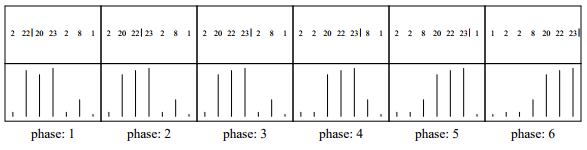
\includegraphics[height=2.5cm,width=13cm]{images/bentleykernighan.png}
\caption{A sequence of stills from an insertion sort algorithm}
\label{fig:bentley-kernighan}	
\end{figure}

Six years later in 1993 Stasko, Badre and Lewis were amongst the first to consider whether algorithm animations assisted learning as much as we might think \cite{StaskoBadreLewis}. Stasko, Badre and Lewis carried out a study which involved attempting to teach two separate groups of students the concept of a ``pairing heap'', with one group using textual descriptions of the algorithm and the other using an animation of the algorithm. Stasko then repeated a similar experiment in 1999 with Byrne and Catrambone. Again, one group used an animation but this time the other group used static diagrams (such as figures from a textbook), instead of textual descriptions like in the previous experiment \cite{StaskoByrneCatrambone}. In both studies the researchers found the results to be disappointing. They found that whilst students in the animation group did perform moderately better than their textual or diagrammatic counterparts, the improvement was not statistically significant.

Despite computer graphic capabilities improving significantly since the 1990s, other more recent studies have shown similar results. The general consensus being that whilst animations do provide a small educational benefit, it is certainly not as large as our intuition would lead us to believe. However, that is not to say that algorithm animations are without use. Stasko, Badre and Lewis suggest that algorithm animations are not particularly effective when students are trying to learn a concept for the first time, but are likely to be much more suitable when students are looking to refine their understanding of a particular notion. The theory is that students should ideally learn the primitive concepts of the algorithm using conventional methods initially, then transition to using animations when looking to clarify and solidify their understanding of certain aspects.

Stasko, Badre and Lewis also reveal a list of guidelines they believe to be effective advice when building algorithm animations, some of which are summarised below:
\begin{itemize}
\item The animation should be augmented with textual descriptions.
\item The animation should include rewind-replay capabilities.
\item Students should be able to build the animation themselves.
\end{itemize}
These guidelines suggest that algorithm animations require accompanying messages that explain the logic of the algorithm at each step. Also, the animation should be interactive in order to engage students in ``active learning'' over ``passive learning''. This interactivity would include intricate controls over the playback of the animation and the ability to modify the input of the algorithm.

\section{Existing Products}
Currently, very few existing tools provide even static illustrations of compilation components (such as syntax trees) and virtually no tools exist that create animations of the compilation process as a whole. There are however, an abundance of web applications that animate more straightforward algorithms, such as sorting or searching algorithms. 

One of the most popular and well implemented is VisuAlgo \cite{visualgo}. VisuAlgo provides an interface for animating various sorting algorithms, including bubble sort, selection sort, etc. As shown in Figure \ref{fig:visualgo}, VisuAlgo implements many of the guidelines we previously listed. It provides impressive playback controls, the ability to choose the input of the algorithm and displays in-depth descriptions of the algorithm's current progress in both plain English and pseudo-code. 

\begin{figure}
	\centering
	\begin{subfigure}[b]{0.45\textwidth}
		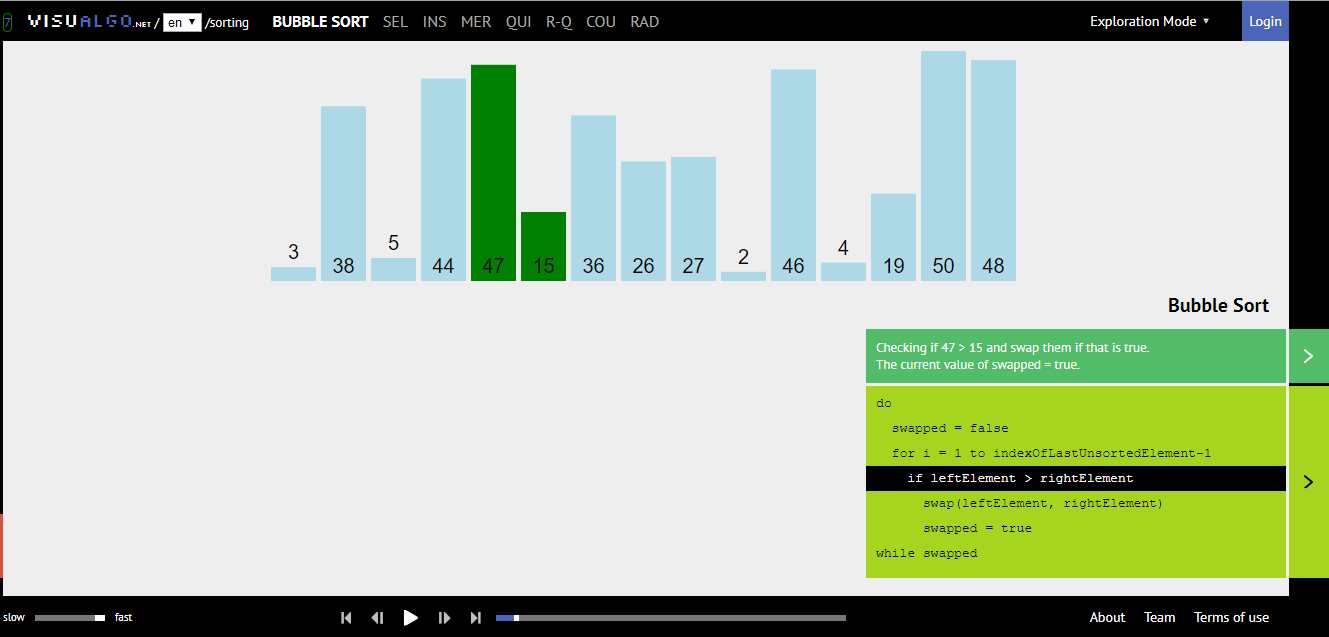
\includegraphics[height=4cm,width=\linewidth]{images/visualgo.png}
		\caption{VisuAlgo}
		\label{fig:visualgo}
	\end{subfigure}
	~
	\begin{subfigure}[b]{0.45\textwidth}
		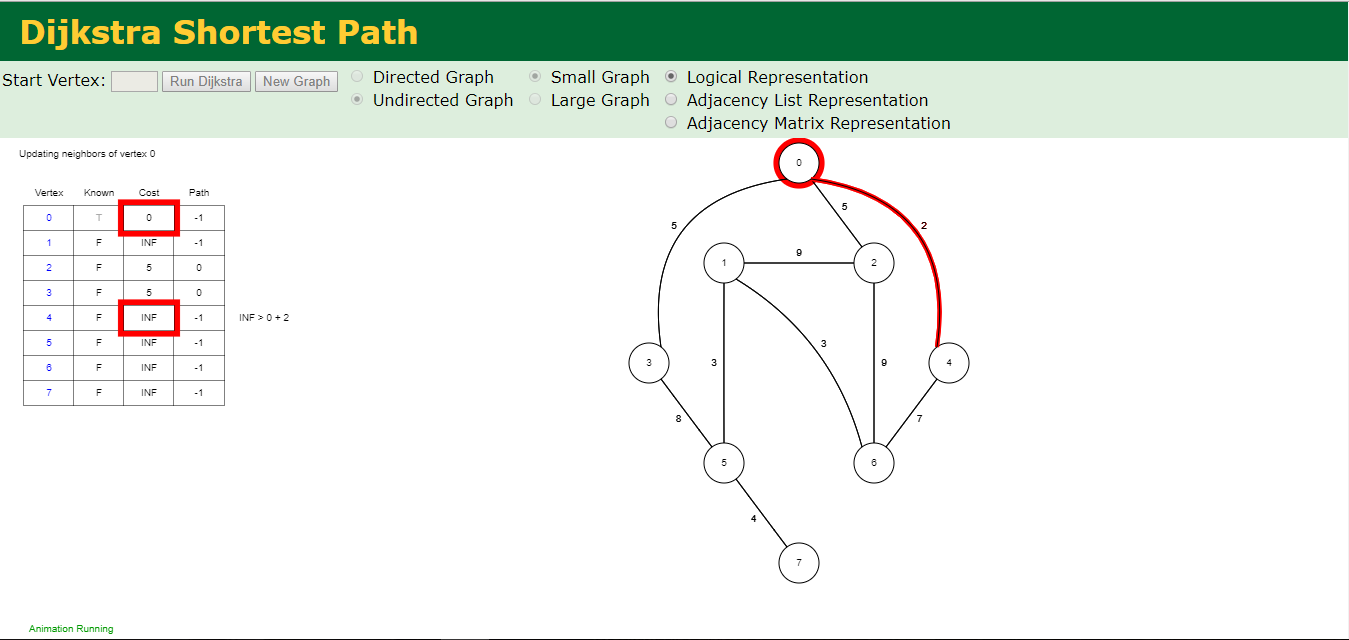
\includegraphics[height=4cm,width=\linewidth]{images/dijkstra.png}
		\caption{The University of San Francisco}
		\label{fig:dijkstra}
	\end{subfigure}
	\caption{Animations of different algorithms from different applications}\label{fig:visualgo-dijkstra}	
\end{figure}


Departing from pure sorting algorithms, the University of San Francisco developed a small web application which animates Dijkstra's algorithm \cite{dijkstra}, as shown in Figure \ref{fig:dijkstra}. Dijkstra's algorithm is arguably more complicated than most sorting algorithms, involving the need to visualise tables and graphs. However, we see that at the expense of this complexity, the application has sacrificed several usability aspects in comparison to VisuAlgo. You cannot define your own input and you cannot pause or rewind the animation. Additionally, whilst some very primitive details are displayed next to the table at each stage, they are far from informative explanations. 

\section{Discussion}
Despite studies showing that algorithm animation is not as effective as we might have initially believed, it would seem that the surprisingly poor performance is due to specific circumstances which could be alleviated if the environment in which an algorithm animation tool was targeted for use was selected more carefully. 

The studies found that algorithm animation was less effective when applied to novice students who were learning the algorithms for the first time, yet could be an effective tool for students who are looking to revise particular concepts. Consequently, any future algorithm animation tool should likely act as a secondary learning resource. Ideally, students should have been taught the concepts using conventional methods to begin with, then the educator can distribute the application to students who can utilise this as a means to refine and clarify understanding.

When considering the previous guidelines proposed by Stasko, Badre and Lewis and how they might affect algorithm animation software, it appears a potential system should:
\begin{itemize}
\item Provide supplementary textual explanations that rationalise and justify the logic of the algorithm.
\item Include rewind-replay functionality that allows the animation to be restarted, or played step-wise, backwards and forwards.
\item Ensure users can create the animation themselves by allowing them to modify the input to the algorithm.
\end{itemize}

% Feel I should remove these last 2 paragraphs but unsure how else to discuss existing products.
After analysing some examples of current products that are available in the area of algorithm animation, such as VisuAlgo and the University of San Francisco's Dijkstra's algorithm animator, it seems there is a trade-off between complexity and usability. In order to animate a considerably more complex algorithm, the University of San Francisco sacrifices much of the visual support and playback control that VisuAlgo is able to provide. 

However, a tool based on compiler animation would need to include both aspects of complexity and usability. The tool would implement an algorithm that is certainly more complex and volatile than even Dijkstra's algorithm, but in order to be educationally effective, it also needs to provide the display of highly input-dependent analytics and implement the usability and interactivity features such as playback control that are embedded within the guidelines of the previous studies.

\chapter{The Fun Programming Language \& Compilation Theory}
This chapter aims to introduce the reader to the main tools and concepts used throughout this dissertation. Firstly, we begin with a small overview of the Fun programming language and its main features. Secondly, we consider how and why compilers parse source code into syntax trees and why some representations of a syntax tree might be more beneficial than others. Thirdly, we take an in-depth look at the three main phases of compilation: syntactic analysis, contextual analysis and code generation; the latter two of which form the animation basis of this project. Finally, we discuss the use of code templates as a theoretical tool for assisting compiler developers in deciding which object code to generate for various constructs within a programming language.

\section{The Fun Programming Language}
Included in Niklaus Wirth's 1975 book {\it Algorithms + Data Structures = Programs}, was a language written entirely in Pascal named ``PL/0'' which was intended as a small educational programming language, used to teach the concepts of compiler construction. The language contains very primitive constructs and limited operations. Similarly to PL/0, ``Fun'' is a simple imperative language built using Java and ANTLR \cite{antlr}, developed at Glasgow University by David Watt and later extended by Simon Gay. Its purpose is to exhibit various general aspects of programming languages, including the construction of an elementary compiler. The language is provided as a supplementary aid during the delivery of the level 3 computer science course, {\it Programming Languages}, at Glasgow University.

Fun has variables, procedures and functions. Variables can have a declared type of \texttt{int} or \texttt{bool} only. All variables must be initialised with an expression of the same type upon declaration. Procedures have type \texttt{T $\rightarrow$ void} and functions have type \texttt{T $\rightarrow$ T'}. \texttt{T} represents the type of an optional parameter. Procedures return no value (hence \texttt{$\rightarrow$ void}) and functions must return a value of the type \texttt{T'} (hence \texttt{$\rightarrow$ T'}). Fun has one predefined function and one predefined procedure: \texttt{read} and \texttt{write}. \texttt{read()} is a function that returns user input as an integer and \texttt{write(\textbf{int} n)} is a procedure that writes the value of \texttt{n} to standard output. Below is an example of a Fun program which utilises variables, functions and procedures to calculate and output the factorial value of user input:
\begin{alltt}
\textbf{bool} verbose = true

\textbf{func int} fact(\textbf{int} n):    
    \textbf{int} f = 1   
    \textbf{while} n > 1:    
        f = f*n   
        n = n-1  .   
    \textbf{return} f  
.  

\textbf{proc} main():  
    \textbf{int} num = read()   
    \textbf{while not} (num == 0):    
        \textbf{if} verbose: write(num) .    
        write(fac(num))    
        num = read() .  
.
 \end{alltt}
 
Similarly to other languages, the entry-point of a Fun program is the \texttt{main()} procedure. In this example, \texttt{main()} begins by reading a number from user input. If the number is 0 the program terminates, otherwise, if the boolean variable \texttt{verbose} is set to \texttt{true}, \texttt{main()} writes the number to standard output and then passes the number to the \texttt{fact()} function. \texttt{fact()} iteratively calculates and returns the factorial value of its input argument \texttt{n}. \texttt{main()} then writes the factorial value to standard output and requests another number from the user.
 
The Fun programming language has a \textit{\textbf{flat block structure}}. A flat block structure means that variables may reside in either a local or a global scope, and that the same identifier may be declared locally and globally. Since functions and procedures cannot be defined within other functions and procedures, they are always global. A variable that is declared as a parameter of or declared within a function/procedure is considered local. Variables declared outside of any function/procedure are considered global. In the example above, we note that \texttt{verbose} is a global boolean variable, whereas \texttt{n} and \texttt{f} are integer variables local to the function \texttt{fact}.

Whilst Fun may differ significantly from other programming languages, particularly in its complexity, it is not the case that the notions it aims to represent are exclusive to the Fun language or the Fun compiler. Fun is sufficiently generic that the core concepts of compiler theory can be delivered in a simple, comprehensible format (due to the simplicity of the language), which then facilitates learners in applying the same logic to more complex constructs in other languages.

\section{Syntax Trees}
During compilation, a source program is parsed into a \textit{\textbf{syntax tree}}. A syntax tree is a hierarchical syntactic representation of a source program; with top-level statements nearer the root, and more deeply nested statements nearer the leaves. We typically consider two types of syntax tree: the \textit{\textbf{parse tree}} (sometimes called a concrete syntax tree) and the \textit{\textbf{abstract syntax tree}} (AST). Translating a source program into a syntax tree means the compiler can more easily reason about the underlying structure and grammatical nature of the program, which is necessary for certain stages of compilation.

A parse tree retains all information about a program, including the information that may appear to be unnecessary, such as white-space and parentheses. Conversely, an AST is a smaller, more concise adaptation of the parse tree. An AST usually ignores redundant details which are derivable from the shape of the tree. Figure \ref{fig:parse-abstract-tree} demonstrates the visual differences between a parse tree and an AST of the same hypothetical Fun program. 

\begin{figure}[h]
	\begin{subfigure}[b]{0.5\textwidth}
		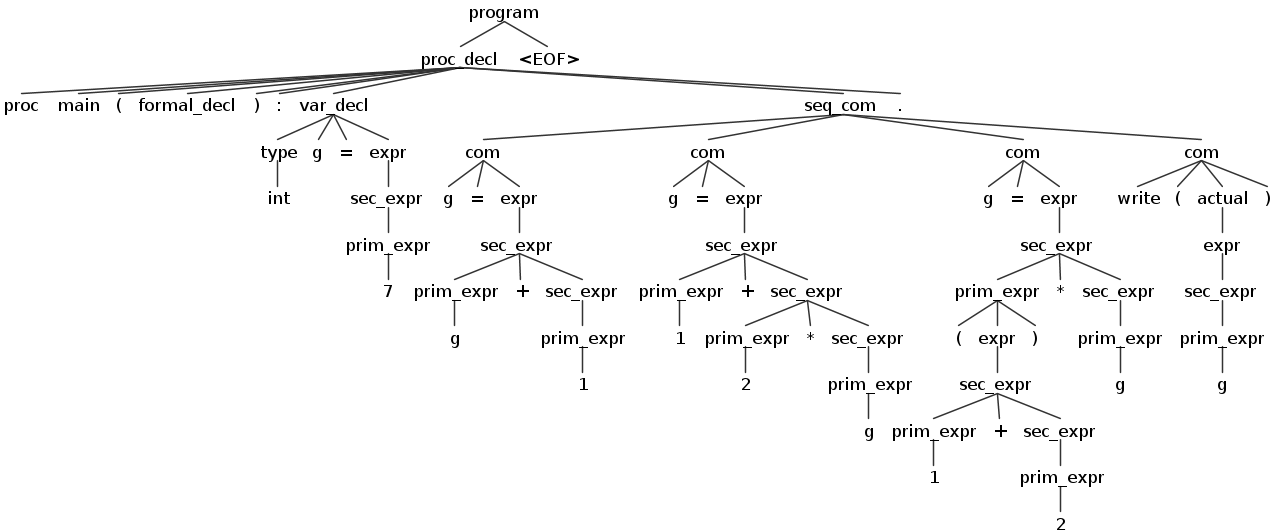
\includegraphics[height=5.5cm,width=\linewidth]{images/2-2a.png}
		\caption{Parse tree}
		\label{fig:ANTLR-parse-tree}
	\end{subfigure}
	\begin{subfigure}[b]{0.5\textwidth}
		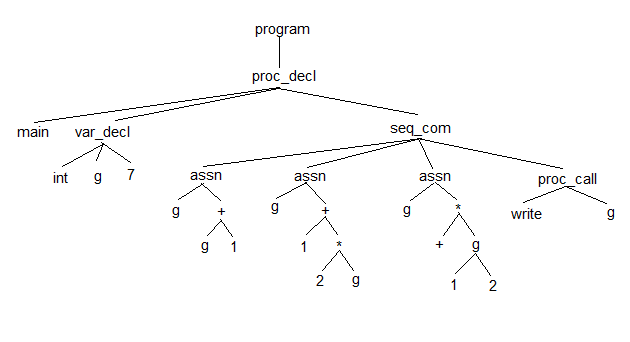
\includegraphics[height=5.5cm,width=\linewidth]{images/2-2b.png}
		\caption{Abstract syntax tree}
		\label{fig:ANTLR-syntax-tree}
	\end{subfigure}
	\caption{Parse tree and AST of the same hypothetical Fun program}\label{fig:parse-abstract-tree}	
\end{figure}

At the initial stages of compilation, the compiler will attempt to translate the input program into either a parse tree or an AST. The generated tree is then traversed during contextual analysis and code generation, which is described in detail in Section 3.3. How the compiler chooses to visit each node in the tree during the traversal is language-dependent, but the semantics are vaguely similar to that of a depth-first traversal. 

Since ASTs are usually much smaller and less crowded than their parse tree counterparts, they are often far easier to read and understand. Any information that is lost from the conversion of a parse tree to an AST is usually semantic and does not affect how the syntax tree would be evaluated. Consequently, when trying to illustrate syntax tree concepts to students from an educational perspective, we generally prefer to use visualisations of ASTs over parse trees.

\section{Compilation Phases}
In general, compilation is the process of automatically translating high-level code into low-level code. The most common case is to convert a program whose source code is written in some programming language, into an executable program. This compilation process can usually be decomposed into three distinct phases: 
\begin{enumerate}[label=\alph*)]
\item \textit {Syntactic Analysis}
\item \textit {Contextual Analysis}
\item \textit {Code Generation}
\end{enumerate}
If either syntactic or contextual analysis encounters an error (as determined by the language's specification) during its execution, the phase completes, but the remainder of the compilation process is halted and the errors are reported to the programmer. Note that the following subsections assume the compiler is employing an AST representation of a syntax tree. See Figure \ref{fig:compilation-pipeline} for a diagram of a typical compilation pipeline.

\begin{figure}[h]
\centering
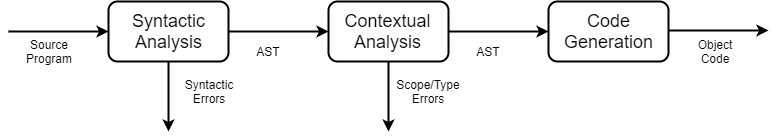
\includegraphics[scale=0.5]{images/3-2a.png}
\caption{Compilation Pipeline}
\label{fig:compilation-pipeline}	
\end{figure}

\subsection{Syntactic Analysis}
Syntactic analysis takes a source program as input and upon success, produces an AST. The purpose of syntactic analysis is to verify whether the source program is well-formed in accordance to the source language's syntax rules. Syntactic analysis can be broken down into \textit{\textbf{lexing}} and \textit{\textbf{parsing}}.

Lexing is the process of breaking down an input program into a stream of \textit{\textbf{tokens}}. A token is simply a single element of the input program. For example, a token could be an individual identifier, operator or keyword. How the compiler chooses to define tokens is dependent upon the implementation of the language. The token stream is then passed as input to the parser. Figure \ref{fig:token-stream} shows how a small excerpt of code may be decomposed into a token stream.

\begin{figure}[h]
\centering
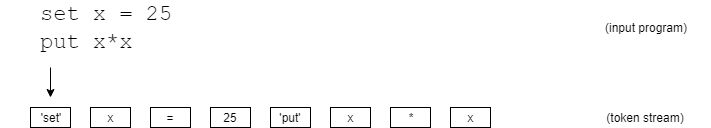
\includegraphics[scale=0.5]{images/token_stream.png}
\caption{Lexing of source code into a token stream}
\label{fig:token-stream}	
\end{figure}

A parser converts a token stream into an AST using some parsing algorithm. The Fun compiler uses \textit{\textbf{recursive-descent}} parsing. Recursive-descent parsing involves ``consuming'' the token stream from left to right. At each token, the parser checks whether the next sequence of tokens are of the correct type, as determined by the language's syntax. The parser carries out this check for every token in the stream. If any checks fail, a syntax error is reported to the programmer. If all tokens are consumed successfully, the parser outputs an AST representing the parsed program.

\subsection{Contextual Analysis}
Upon successful completion of syntactic analysis, the generated AST is traversed  by a contextual analyser. A contextual analyser checks whether the source program represented by the AST conforms to the source language's scope and type rules. Contextual analysis utilises an auxiliary data structure called a \textit{\textbf{type table}} in order to help carry out these checks. Each row of the type table contains three fields of information about a declared variable: its scope (which as discussed in Section 3.1 can be local or global), its identifier and its type. Figure \ref{fig:type-table} demonstrates a small example. The table reveals that the corresponding program contains two integer variables with the identifier \texttt{x} (globally and locally defined) and a global procedure with the identifier \texttt{main} which takes no parameters and returns no value. Contextual analysis can be broken down into \textit{\textbf{scope checking}} and \textit{\textbf{type checking}}.

\begin{figure}[h]
\centering
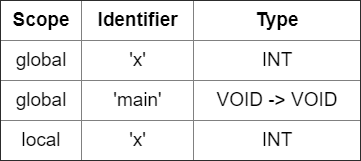
\includegraphics[scale=0.5]{images/type-table.png}
\caption{Type Table}
\label{fig:type-table}	
\end{figure}

Scope checking ensures that every variable used in the program has been previously declared. If the contextual analyser encounters the \textit{declaration} of an identifier as it is traversing over the AST, it inserts the identifier along with its scope and type into the type table. If the contextual analyser finds that there is already an entry in the table with the same scope and identifier, then a scope error is reported to the programmer. Similarly, if the contextual analyser encounters the \textit{usage} of an identifier during the traversal, it checks that the identifier is already in the type table (i.e., has been previously declared). If the identifier cannot be found in the type table, then a scope error is reported to the programmer. Figure \ref{fig:variable-decl-use} shows two ASTs that illustrate the declaration and usage (assignment) of a variable \texttt{n}. The variable \textit{declaration} construct in Figure \ref{fig:variable-decl} would lead the compiler to insert a row into the type table with values: \texttt{[global, n, INT]}. The variable \textit{assignment} construct in Figure \ref{fig:variable-use} would lead the compiler to lookup entries in the type table with identifier \texttt{n} to ensure the variable has been previously declared before attempting to assign a new value to it.

\begin{figure}[h]
	\centering
	\begin{subfigure}[b]{0.3\textwidth}
		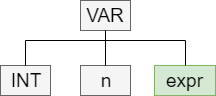
\includegraphics[scale=0.65]{images/variable-decl.png}
		\caption{Variable declaration}
		\label{fig:variable-decl}
	\end{subfigure}
	~
	\begin{subfigure}[b]{0.3\textwidth}
		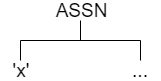
\includegraphics[scale=0.65]{images/variable-use.png}
		\caption{Variable usage}
		\label{fig:variable-use}
	\end{subfigure}
	\caption{ASTs demonstrating the declaration and usage of a variable \texttt{n} (assuming global scope)}\label{fig:variable-decl-use}	
\end{figure}

Type checking ensures that every operation in the program has operands of the expected type. The rules the contextual analyser uses to determine if an operation has the ``correct'' operands vary from construct to construct. For example, referring back to Figure \ref{fig:variable-use}, we see the construct for variable assignment. In this case, we are assigning the value of some expression, represented by \texttt{expr}, to the variable \texttt{n}. When the contextual analyser encounters this construct during the traversal, it will retrieve the type of \texttt{n} from the type table, then traverse the expression \texttt{expr} to determine its type. The contextual analyser will then check that the type of \texttt{expr} is the same as the type of \texttt{n}. For example, given that in Figure \ref{fig:variable-decl} \texttt{n} was defined as an integer, \texttt{x = 5 + 10} would be a valid assignment, whereas \texttt{x = false} would result in a type error.

\subsection{Code Generation}
Upon successful completion of contextual analysis, the generated AST is traversed by a code generator. A code generator translates the source program into a lower level language, such as assembly language or object code. Code generation utilises an auxiliary data structure called an \textit{\textbf{address table}}. Each entry in the address table contains three fields of information about a declared variable: its scope, its identifier and its address. Figure \ref{fig:address-table} demonstrates a small example. The table reveals how each identifier has been allocated an address in the address space belonging to either local or global variables. Code generation can be broken down into \textit{\textbf{address allocation}} and \textit{\textbf{code selection}}.

\begin{figure}[h]
\centering
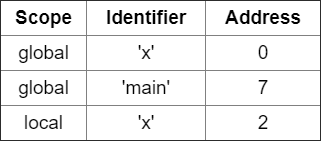
\includegraphics[scale=0.5]{images/address-table.png}
\caption{Address Table}
\label{fig:address-table}	
\end{figure}

Address allocation decides the representation and address of each variable in the source program. If the code generator encounters the declaration of an identifier as it is traversing over the AST, it determines a suitable address which it inserts into the address table along with the corresponding identifier and scope. In the case of Fun, all variables conveniently have a size of 1, meaning the compiler can simply allocate incrementally consecutive addresses to each variable as it is encountered.

Code selection selects and generates the final object code. The developer of the compiler should plan which object code is selected for each construct encountered within the AST. The developer does this by devising a \textit{\textbf{code template}} for each construct in the language.

\section{Code Templates}
When developing a compiler, it is important to consider how each construct in the underlying language should be translated into object code. A code template provides a means of creating a theoretical model for each construct that specifies how the corresponding object code should be selected. Each template is often just a list of directives (written in plain English) that specifies which object code instructions to emit and defines how any constituent expressions/commands of the construct should themselves be considered for code selection. 

For example, on the left-side of Figure \ref{fig:plus} we see an AST that demonstrates the addition of two expressions, where \texttt{expr1} and \texttt{expr2} are sub-expressions of the \texttt{PLUS} construct. Of course, the value of the two expressions must be calculated before attempting to add the two together. In other words, the compiler must evaluate \texttt{expr1} and \texttt{expr2} and emit the object code to load those values into memory \textit{before} emitting the addition object code. Therefore, the code template for the \texttt{PLUS} construct should state that \texttt{expr1} and \texttt{expr2} are to be evaluated before we emit any object code to add the expressions together.

On the right-side of Figure \ref{fig:plus} we see an illustration of the code template as described above. Considering each instruction sequentially, it stipulates that firstly we should generate the object code for \texttt{expr1}, then \texttt{expr2}. Only after emitting both instructions that load the value of these expressions into memory can we emit the \texttt{ADD} object code instruction. 

\begin{figure}[h]
	\centering
	\begin{subfigure}[b]{0.3\textwidth}
		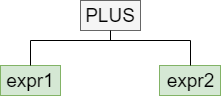
\includegraphics[scale=0.65]{images/plus.png}
	\end{subfigure}
	~
	\begin{subfigure}[b]{0.3\textwidth}
		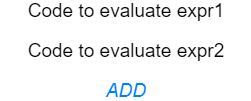
\includegraphics[scale=0.65]{images/plus-template.png}
	\end{subfigure}
	\caption{AST and code template of a \texttt{PLUS} construct}\label{fig:plus}	
\end{figure}

In the general case, it is often true that the compiler may need to translate some (or all) of the constituent statements of a construct into object code before emitting any object code specific to the original construct itself. Unfortunately, how each construct should be evaluated in regards to code generation is not always immediately clear just from the structure of the AST. This is the scenario in which code templates are practical, as they provide a way to exemplify how each construct in the source language should be translated into object code.

\chapter{Requirements}
This chapter initially discusses the methods via which the requirements of this project, which we will henceforth refer to as the \textit{FunCompiler}, were collected and established. The remainder of the chapter lists the FunCompiler's user stories, functional requirements and non-functional requirements.

\section{Methodology}
The requirements of the FunCompiler were elicited through two main techniques. Firstly, through multiple interviews with Simon Gay. Simon is the current lecturer of the Programming Languages course at Glasgow University. Since both the Fun language and the compilation of Fun programs are delivered during the Programming Languages course, students enrolled in this course will naturally be the target user-base of the FunCompiler. Thus, Simon clearly has the expertise and the experience to offer valuable recommendations on the function and operation of the FunCompiler.

The second technique was to simply utilise the insight gained from performing background research. In particular, we strive to ensure the requirements meet the three guidelines we saw in Section 2.1, proposed by Stasko, Badre and Lewis. Below, the three guidelines have been rephrased to apply directly to the FunCompiler:
\begin{enumerate}[label=Guideline \alph*)]
\item Provide supplementary textual explanations that rationalise and justify the logic of the compiler as it visits each node in the AST.
\item Include rewind-replay functionality that allows the compilation animation to be restarted, or played step-wise, backwards and forwards.
\item Ensure users can create the animation themselves by allowing any arbitrary Fun program as input to the compiler.
\end{enumerate}
\pagebreak
\section{User Stories}
After conducting the interviews and the background research, a set of user stories was devised. User stories are short and simple descriptions of a feature, told from the perspective of a potential user:\\
\begin{table}[h]
\centering
\begin{tabular}{@{}cl@{}}
\toprule
\multicolumn{1}{l}{\textbf{User Story}} & \textbf{Description} \\ \midrule
\textbf{1} & \begin{tabular}[c]{@{}l@{}}As a user, I want to read details of the Fun language, so that I can write \\ valid Fun programs as input and better understand the compilation animations.\end{tabular} \\\\
\textbf{2} & \begin{tabular}[c]{@{}l@{}}As a user, I want to be able to input any Fun program, so that I can learn \\ about the compilation process in the general case, not just for specific examples.\end{tabular} \\\\
\textbf{3} & \begin{tabular}[c]{@{}l@{}}As a user, I want to be able to view the animation of the contextual analysis \\ phase of my program, so that I can understand how the compiler carries out this task.\end{tabular} \\\\
\textbf{4} & \begin{tabular}[c]{@{}l@{}}As a user, I want to be able to view the animation of the code-generation\\ phase of my program, so that I can understand how the compiler carries out this task.\end{tabular} \\\\
\textbf{5} & \begin{tabular}[c]{@{}l@{}}As a user, I want to be able to play different sections of the compilation \\ animation independently (i.e., contextual analysis or code generation), \\ so that I can focus my learning on specific areas.\end{tabular} \\\\
\textbf{6} & \begin{tabular}[c]{@{}l@{}}As a user, I want to be able to see textual descriptions that explain what \\ the compiler is doing at each stage of the animation, so that I can \\ better understand the logic of the compiler.\end{tabular} \\\\
\textbf{7} & \begin{tabular}[c]{@{}l@{}}As a user, I want to be able to see any supplementary information or feedback \\ (including address/type tables, code templates and generated \\ object code), so that I get all the information available in order to help \\ further my understanding.\end{tabular} \\\\
\textbf{8} & \begin{tabular}[c]{@{}l@{}}As a user, I want to be able to replay an animation, so that I can review \\ any details I missed/misunderstood.\end{tabular} \\\\
\textbf{9} & \begin{tabular}[c]{@{}l@{}}As a user, I want to be able to step through the animation at my own \\ pace, so I can more easily understand what is happening during the animation.\end{tabular} \\ \bottomrule \\
\end{tabular}
\end{table}

\section{Functional Requirements}
After creating user stories and using any previous research, a formal list of functional requirements was created. Functional requirements are intended to capture a specific function of a system:

\begin{table}[]
\centering
\begin{tabular}{@{}cl@{}}
\toprule
\multicolumn{1}{l}{\textbf{\begin{tabular}[c]{@{}l@{}}Functional \\ Requirement\end{tabular}}} & \textbf{Description} \\ \midrule
\textbf{1} & Allow users to input any arbitrary Fun program as input to the compiler animator. \\\\
\textbf{2} & Allow users to animate either contextual analysis or code generation separately. \\\\
\textbf{3} & Display the generated AST that represents the input Fun program. \\\\
\textbf{4} & \begin{tabular}[c]{@{}l@{}}Enable a controllable animation over this AST representing one of the two \\ phases (contextual analysis or code generation).\end{tabular} \\\\
\textbf{5} & At each step of the animation, highlight the corresponding node in the AST. \\\\
\textbf{6} & Allow users to play the animation continuously. \\\\
\textbf{7} & Allow users to pause the animation. \\\\
\textbf{8} & Allow users to move forwards through the animation, one step at a time. \\\\
\textbf{9} & Allow users to move backwards through the animation, one step at a time. \\\\
\textbf{10} & \begin{tabular}[c]{@{}l@{}}At each step of the animation, display messages that explain the logic of\\ the compiler, i.e., what it is currently doing, or what it is going to do.\end{tabular} \\\\
\textbf{11} & \begin{tabular}[c]{@{}l@{}}At each step of the animation, display the type table (if contextual analysis) \\ or the address table (if code generation) in its current state during the \\ compilation.\end{tabular} \\\\
\textbf{12} & During code generation, display the code template of each node as it is visited. \\\\
\textbf{13} & \begin{tabular}[c]{@{}l@{}}During code generation, display the emitted object code in its current state during\\ the compilation.\end{tabular} \\\\
\textbf{14} & \begin{tabular}[c]{@{}l@{}}If a user inputs a syntactically invalid Fun program, prevent the animation and\\ report the errors to the user.\end{tabular} \\\\
\textbf{15} & \begin{tabular}[c]{@{}l@{}}If a user inputs a contextually invalid Fun program, allow animation of the\\ contextual analysis phase but disallow animation of the code generation \\ phase and report the errors to the user.\end{tabular} \\\\
\textbf{16} & \begin{tabular}[c]{@{}l@{}}Make the full specification of the Fun language available within the web\\ application.\end{tabular} \\ \bottomrule
\end{tabular}
\end{table}

Along with implementing the core functionality of a compiler animator (along with a few extra features), it is clear to see from functional requirements \textbf{1}, \textbf{6}, \textbf{7}, \textbf{8}, \textbf{9} and \textbf{10}, that we have more than comfortably included the elements necessary to satisfy guidelines a), b) and c).

\section{Non-functional Requirements}
In contrast to functional requirements that detail specific behaviours of a system, non-functional requirements often consider overall utilities of a system, such as security, usability and extensibility:\\
\begin{table}[h]
\centering
\begin{tabular}{@{}cl@{}}
\toprule
\multicolumn{1}{l}{\textbf{\begin{tabular}[c]{@{}l@{}}Non-Functional \\ Requirement\end{tabular}}} & \textbf{Description} \\ \midrule
\textbf{1} & The application must work on all modern browsers. \\\\
\textbf{2} & \begin{tabular}[c]{@{}l@{}}The application must be able to interact efficiently with a Java-based \\ application (the Fun compiler).\end{tabular} \\\\
\textbf{3} & The application must be responsive, at least to a tablet level. \\\\
\textbf{4} & The application must ensure no malicious code can be executed \\ \bottomrule
\end{tabular}
\end{table}

\section{Analysis}
In overview, a typical workflow for the FunCompiler might look as follows: firstly, the user arrives at the website and should be able to view the specification of Fun language before needing to use the animator. Then, the user can type a Fun program into some kind of code editor and choose to animate either contextual analysis or code generation. At this point, if there were any syntactic or contextual errors, they would be reported to the user using the semantics as defined above.

After selecting one of the two phases, the AST that represents the input program is displayed on screen along with playback buttons (play, pause, forwards, backwards). As the animation progresses, nodes within the AST are highlighted to symbolise the current progress of the compiler. As each node is highlighted, detailed information as described above is simultaneously displayed elsewhere on screen. The user is of course free to pause the animation to review the current information displayed, or rewind to review. At any point the user may modify the current input Fun program and select either the same or a different compilation phase, which will halt any current animations.

This potential workflow of the FunCompiler is enough to meet all functional requirements. The non-functional requirements cover issues that are strictly more technical, the solutions to which will be discussed during the system design and the physical implementation.

\chapter{Design}
This chapter covers the aesthetic design process of the FunCompiler. We develop simple low-fidelity wireframe designs of the individual components of the user interface and consider how each of these different components might satisfy our functional requirements. We then look at a more complete design of the user interface and observe how a user might transition from page to page. %Finally, in order to make the website compatible across different screen sizes, we consider a responsive design of the application.

\section{Application Interface}
To act as the first step in realising the project's functional requirements, we develop a series of quick and primitive low-fidelity wireframe designs, each representing an individual component of the user interface. Detailed below are a set of five interface components which when combined satisfy the majority of the application's functional requirements. Each component consists of a wireframe design and considers how the component may meet one or more of the functional requirements (FRs).

\subsection{Code Editor}
The code editor will be the text-area in which users are able to enter code written in the Fun language (FR \textbf{1}). Ideally, the code editor should follow some of the semantics of standard programmatic text editors, including syntax highlighting and auto-indention. Notice that in Figure \ref{fig:code-editor-wireframe} two buttons for ``Contextual Analysis'' and ``Code Generation'' have been attached to the bottom of the code editor. These buttons will trigger the transmission of the input code to the compiler and thus initiate the corresponding animation (FR \textbf{2}).

\begin{figure}[h]
\centering
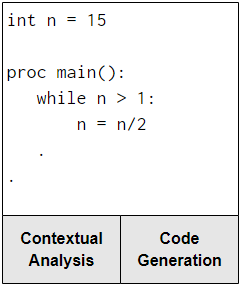
\includegraphics[scale=0.6]{images/code-editor-wireframe.png}
\caption{Code editor wireframe}
\label{fig:code-editor-wireframe}	
\end{figure}

\subsection{AST}
The AST of the input program is the foundation of the animation. The AST will be displayed in the conventional hierarchical tree format where the animator will highlight each node consecutively, corresponding to the progress of the compiler (FR \textbf{3, 5}). For example, along with showing the general structure of the AST for a Fun program, Figures \ref{fig:anim-step-1} to \ref{fig:anim-step-3} demonstrate how the application might animate the AST. At each ``step'' of the animation, the next node in the traversal is highlighted, whilst the previous node is returned to its original state.

\begin{figure}[h]
	\centering
	\begin{subfigure}[b]{0.3\textwidth}
		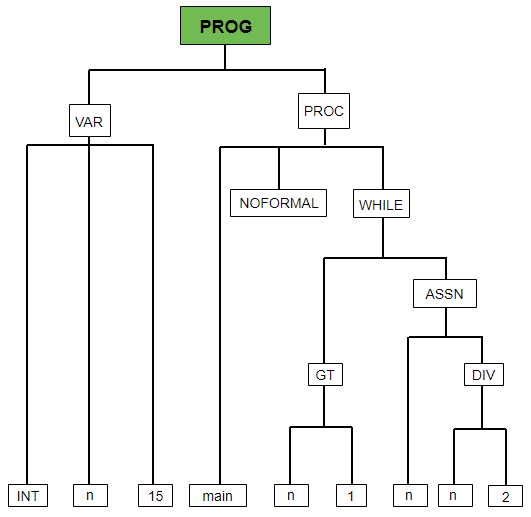
\includegraphics[width=\linewidth]{images/animation-active-wireframe.png}
		\caption{Step 1 of animation}
		\label{fig:anim-step-1}
	\end{subfigure}
	~
	\begin{subfigure}[b]{0.3\textwidth}
		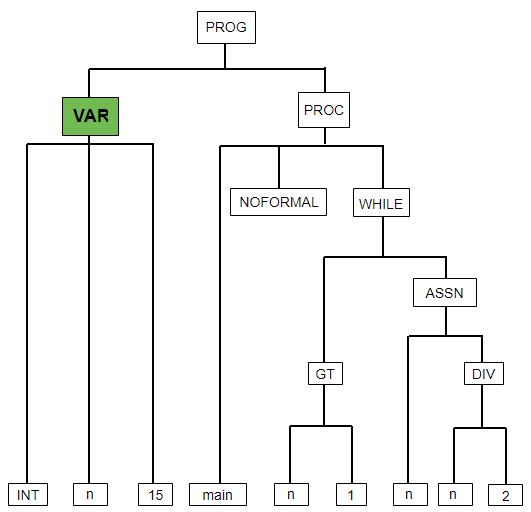
\includegraphics[width=\linewidth]{images/animation-active-wireframe2.png}
		\caption{Step 2 of animation}
		\label{fig:anim-step-2}
	\end{subfigure}	
	~
	\begin{subfigure}[b]{0.3\textwidth}
		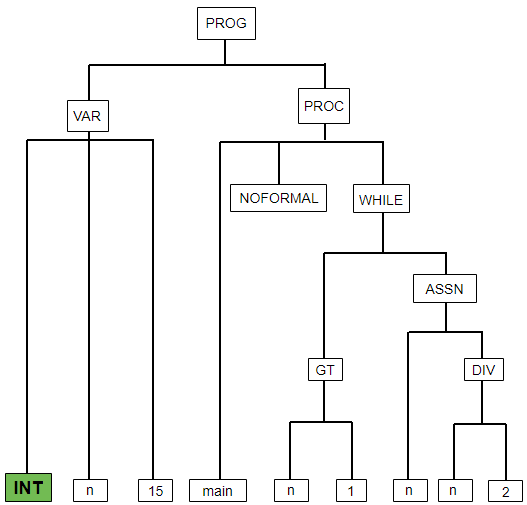
\includegraphics[width=\linewidth]{images/animation-active-wireframe3.png}
		\caption{Step 3 of animation}
		\label{fig:anim-step-3}
	\end{subfigure}	
	\caption{AST wireframes}
	\label{fig:animation-active-wireframe}	
\end{figure}

\subsection{Augmentations}
As the compiler traverses the tree, the application should augment the animation with any supplementary information that may aid the user's understanding of the compilation, including explanatory messages, type/address tables, code templates and object code. We henceforth collectively refer to each of these factors as ``augmentations''. Figure \ref{fig:analytics-ca-wireframe} illustrates the augmentations required for contextual analysis, including a type table and a section to display explanatory messages (FR \textbf{10, 11}). Figure \ref{fig:analytics-cg-wireframe} illustrates similar augmentations for code generation, with the type table replaced by an address table and two added sections to display code templates and object code (FR \textbf{12, 13}). Note that all augmentations, other than tables, are just textual descriptions/lists, and hence are simply represented as labelled areas in the following wireframes.

\begin{figure}[h]
	\centering
	\begin{subfigure}[b]{0.3\textwidth}
		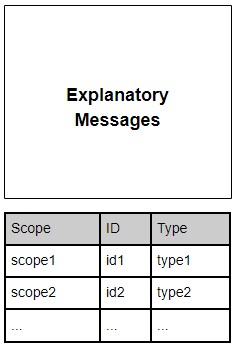
\includegraphics[scale=0.6]{images/analytics-ca-wireframe.png}
		\caption{Contextual analysis augmentations}
		\label{fig:analytics-ca-wireframe}
	\end{subfigure}
	~
	\begin{subfigure}[b]{0.3\textwidth}
		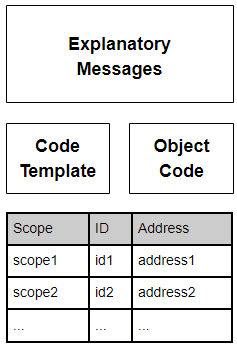
\includegraphics[scale=0.6]{images/analytics-cg-wireframe.png}
		\caption{Code generation \\ augmentations}
		\label{fig:analytics-cg-wireframe}
	\end{subfigure}
	\caption{Augmentations wireframe}\label{fig:augmentations-wireframe}	
\end{figure}

\subsection{Playback Controls}
Users require the ability to play, pause and step through (backwards and forwards) the animation. Figure \ref{fig:playback-wireframe} shows two sets of playback buttons (FR \textbf{4}). Intuitively, when the play button is pressed, it should be replaced with the pause button and vice versa. If the user presses the play button, the animator should highlight the next node in the sequence at regular time intervals (for example, each second) (FR \textbf{6}). If the user presses the pause button, the animation should be halted and the currently highlighted node should remain highlighted (FR \textbf{7}). If the user presses the forwards/backwards buttons, this will highlight the next/previous node in the sequence, one node per button press (FR \textbf{8, 9}). If the animation is currently playing when a forwards or backwards button is pressed, it should be implicitly paused.

\begin{figure}[h]
	\centering
	\begin{subfigure}[b]{0.3\textwidth}
		
\includegraphics[]{images/playback-play-wireframe.png}
	\end{subfigure}
	~
	\begin{subfigure}[b]{0.3\textwidth}
		
\includegraphics[]{images/playback-pause-wireframe.png}
	\end{subfigure}
	\caption{Playback controls wireframe}\label{fig:playback-wireframe}	
\end{figure}

\subsection{Fun Specification}
 Figure \ref{fig:fun-specification-wireframe}, illustrates the Fun specification broken down into seven sections. Tabs along the top of the component allow the user to navigate between each section. Each section contains varying amounts of information to explain each concept (FR \textbf{16}).
 
 \begin{figure}[h]
\centering
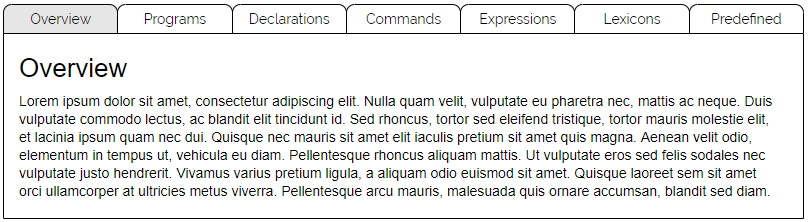
\includegraphics[scale=0.6]{images/specification-wireframe.png}
\caption{Fun specification wireframe}
\label{fig:fun-specification-wireframe}	
\end{figure}

\section{Full Design}
With all necessary components designed, we consider how to combine each of these to create a set of full-sized designs. The presiding design philosophy is that the code editor, the animation and the augmentations are all available within the same view. This is important for two reasons. Firstly, from an educational perspective, there is the obvious necessity that users are able to easily cross-reference between these three components. Secondly, from a usability aspect, as an animation is running, a user should be able to modify the input code and generate a new animation without having the navigate to a different page.

We partition the FunCompiler by splitting the application into three separate pages: the landing page (containing the Fun specification), the contextual analysis animation page and the code generation animation page. We also insert a small navigation bar on each page which includes a link to return to the landing page.

\subsection{Landing Page}
Figure \ref{fig:full1} demonstrates the landing page of the FunCompiler. Here we see that the user has access to the code editor along with access to the full specification of the Fun language. A user can enter a Fun program of their own creation then choose to animate either contextual analysis or code generation by clicking one of the buttons below the code editor.

 \begin{figure}[h]
\centering
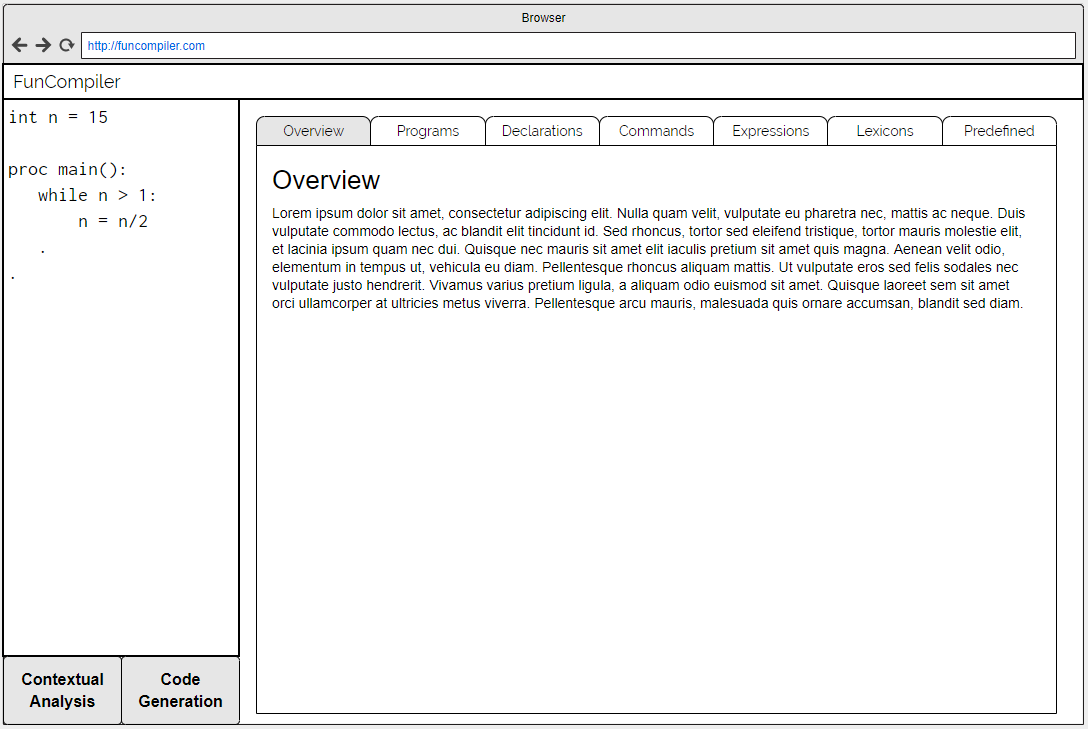
\includegraphics[scale=0.4]{images/full1.png}
\caption{Landing page wireframe}
\label{fig:full1}	
\end{figure}

\subsection{Contextual Analysis Animation Page}
If the user chooses to animate contextual analysis, they are redirected to the page illustrated in Figure \ref{fig:full2}. This page displays an AST generated from the input program, a set of playback controls for the animation, an area to output explanatory messages and a type table. From this page the user still has access to the code editor and is free to modify the input program and generate a new animation. 

 \begin{figure}[h]
\centering
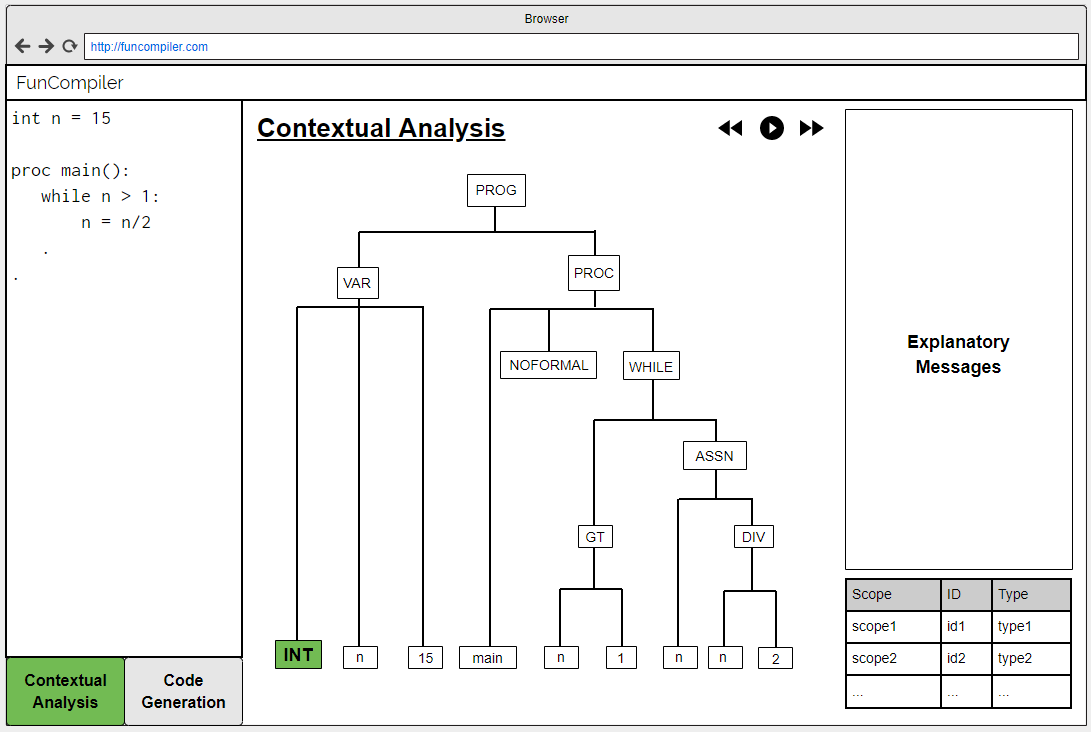
\includegraphics[scale=0.4]{images/full2.png}
\caption{Contextual analysis page wireframe}
\label{fig:full2}	
\end{figure}
\pagebreak
\subsection{Code Generation Animation Page}
If the user chooses to animate code generation, they are redirected to the page illustrated in Figure \ref{fig:full3}. This page displays very similar details to the contextual analysis page, except the type table is swapped for an address table and sections to display code templates and object code have been inserted.

 \begin{figure}[h]
\centering
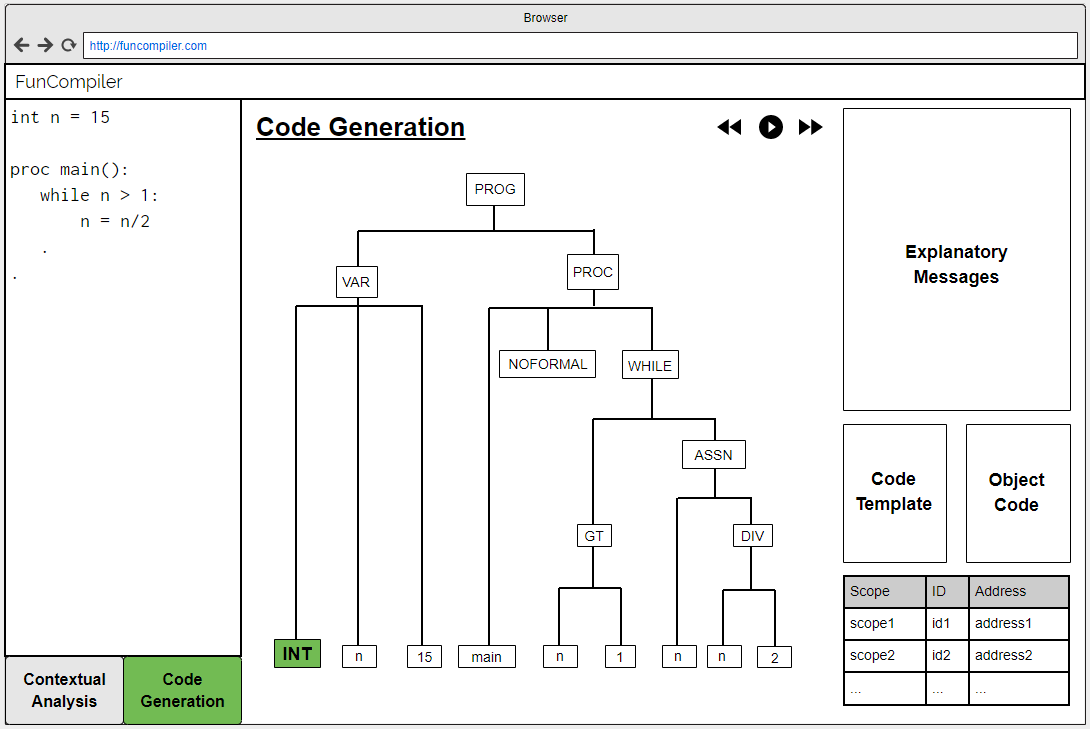
\includegraphics[scale=0.4]{images/full3.png}
\caption{Code generation page wireframe}
\label{fig:full3}	
\end{figure}

\section{Error Handling}
The above component designs successfully covered all but two of the 16 functional requirements. The remaining functional requirements (FR \textbf{14, 15}) are concerned with error handling and preventing certain actions in the event of errors. More specifically, FR \textbf{14} states that we must not allow the animation of either contextual analysis or code generation in the event that the input Fun program contains syntax errors. FR \textbf{15} states that if the input Fun program contains contextual errors, we may animate contextual analysis, but not code generation. In both cases, we present the user with the relevant errors if they try to execute a prohibited action. In order to retain space for the more important aspects of the interface, when a user attempts to submit an invalid program, we simply display the errors in a pop-up window without disturbing the core contents of the page, as illustrated in Figure \ref{fig:syntax-error-wireframe}. With this final addition in place, we have successfully realised all of the FunCompiler's functional requirements.

 \begin{figure}[h]
\centering
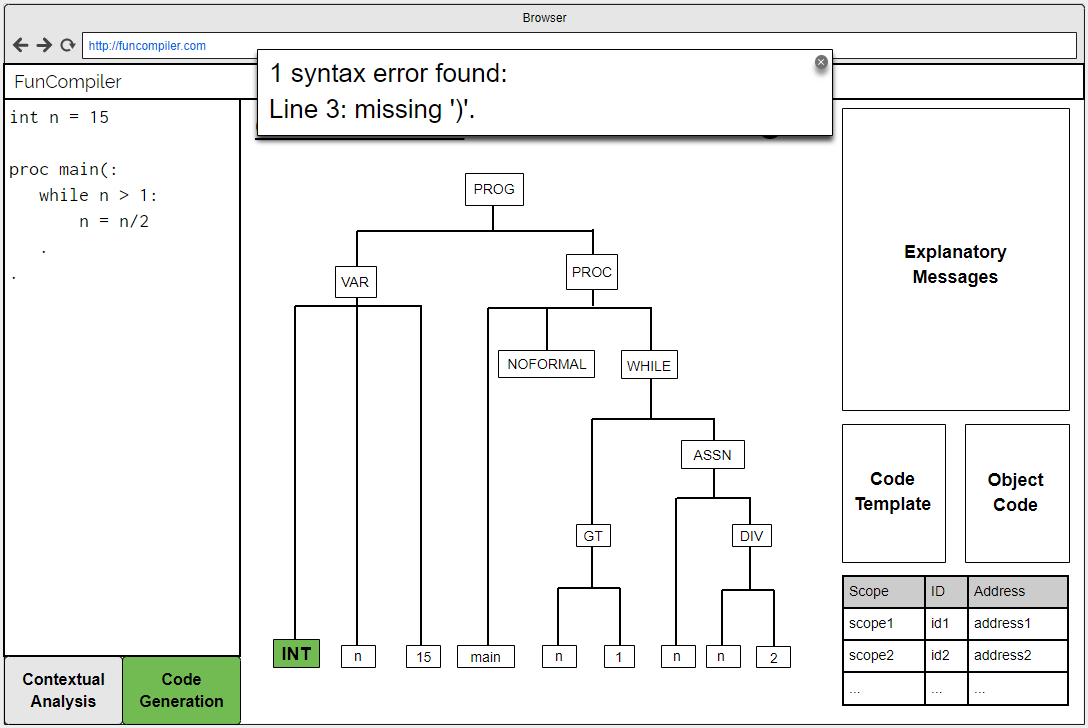
\includegraphics[scale=0.4]{images/syntax-error-wireframe.png}
\caption{Syntax error wireframe}
\label{fig:syntax-error-wireframe}	
\end{figure}

\chapter{System Architecture}
In this chapter we define the system architecture of the FunCompiler. That is, we establish individual system-level components and build a model to specify their organisation/structure, alongside showing the patterns of communication between them.

Firstly, we discuss the differences between a monolithic and a micro-service architecture in regards to web-applications. Secondly, we consider which of these architectures is most applicable to the FunCompiler and how the components of the system will be arranged to fit that model. Finally, using a bottom-up approach we describe the specific technologies that will be used within the FunCompiler, from application-level development frameworks to build tools and packaging systems.

\section{Monolithic vs. Micro-service Architecture}
Traditionally, websites have been built as large, monolithic applications, where each unique service within the website (e.g., authentication, routing, API exposure) is encapsulated under one application, as illustrated in Figure \ref{fig:mono}. Whilst a monolithic architecture may be an appropriate choice for many basic applications, if the system has a diverse range of service implementations, issues are likely to occur.

For example, consider the scenario of a monolithic online shop. Suppose the vast majority of the website's business logic is written in Python but the authentication service is written in PHP. To force the PHP service to operate within a Python environment not only clearly violates the basic principles of a \textit{separation of concerns}, but likely leads to inefficient/insecure methods of communication (e.g., writing/reading from files) and an unscalable, tightly coupled code-base. To solve this issue whilst maintaining a monolithic architecture would require translating the authentication service from PHP to Python, however, this may be undesirable or simply infeasible.

The emerging trend is to extract each of these services out of the main application and allow them to behave as stand-alone components, referred to as micro-services. Figure \ref{fig:micro} demonstrates how a user interacts with the web-application, which in turn communicates with the individual micro-services that have been separated into their own components. Employing a micro-service architecture decouples the services, handles scalability issues with greater ease and allows diversity in programming language or web-framework selection.

\begin{figure}[h]
	\centering
	\begin{subfigure}[b]{0.3\textwidth}
		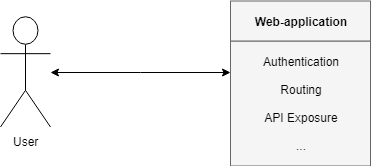
\includegraphics[scale=0.35]{images/mono.png}
		\caption{Monolithic architecture}
		\label{fig:mono}
	\end{subfigure}
	~
	\begin{subfigure}[b]{0.3\textwidth}
		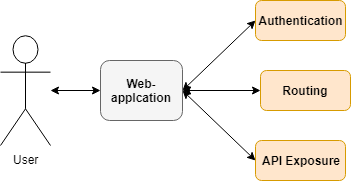
\includegraphics[scale=0.35]{images/micro.png}
		\caption{Micro-service architecture}
		\label{fig:micro}
	\end{subfigure}
	\caption{Monolithic vs. micro-service architecture}\label{fig:mono-micro}	
\end{figure}

\section{FunCompiler Architecture \& Communication}
As discussed in Chapter 3, the compiler of the Fun language is a pre-existing piece of software built with Java and ANTLR. In order to incorporate the compiler within a web-application we have three choices:
\begin{enumerate}[label=\alph*)]
\item Translate the compiler into the same language as used to implement the web-application. 
\item Implement the web-application using a Java-based web-framework.
\item Employ a micro-service architecture, partitioning the FunCompiler into two distinct units: the web-application and the compiler.
\end{enumerate}
Although all choices do essentially produce the same result, choice a) leads to a significant time investment that may produce a weaker implementation of the compiler and choice b) compels us to make a framework selection based on a weak justification. Opting for choice c) means that the compiler does not need to be translated, nor are there any limitations on the choice of web -application framework. Furthermore, even if the compiler and the web-application were natively developed in the same language, choice c) still enforces the most robust separation of concerns.

Following this, we decompose the FunCompiler into two separate components: the web-application and the compiler. The web-application is the user-facing system, serving the web-pages and displaying the animations. The compiler behaves as a micro-service which receives a Fun program as input and outputs the result of the program's compilation (the contents of this result we will discuss more in Section 7.?). 

Of course, the web-application must be able to send user-written Fun programs to the compiler. Likewise, the compiler must be able to return the result of the compilation to the web-application. Therefore, the two components require some method of communication. We do this by exposing the compiler as an API. The API under these circumstances is very simple and requires only one endpoint. 

When a user enters a program within the web-application and chooses to animate either contextual analysis or code generation, the web-application makes an API request to the compiler, sending the input program. When the API receives this request, it passes the program as input to the compiler, executes the compilation and sends a response containing the output back to the web-application. The web-application uses the contents of this response to build the corresponding animation. Figure \ref{fig:funinfra0} illustrates this flow of information.

 \begin{figure}[h]
\centering
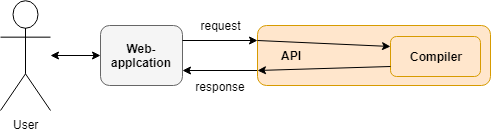
\includegraphics[scale=0.5]{images/funinfra0.png}
\caption{Web-application communicating with the compiler via an API}
\label{fig:funinfra0}	
\end{figure}

\section{Technologies \& Tools}
With the FunCompiler split into its constituent components, we discuss the various system-level technologies and tools that will be used to implement, build and run the application. We start by examining the application-level technologies used by the web-application and the compiler individually, then we consider how to create an abstraction of the system as a whole and package it as a single, portable instance.

\subsection{Web-application Technologies}
\subsubsection{Laravel}
A convenient simplification of the FunCompiler is that the system requires no persistent storage, meaning our system architecture need not include a database. However, even without a database, the web-application is still required to perform a small amount of server-side (or back-end) duties, namely delivering API requests and handling the corresponding responses. We implement this functionality using Laravel, which is an open-source PHP framework intended for the rapid development of web-applications. Like the majority of web-frameworks, Laravel follows a standard \textit{model-view-controller} (MVC) architectural pattern. 

One might argue that given the limited amount of server-side processing required, a relatively large scale framework such as Laravel is excessive. Whilst it's true that a minimalistic framework (i.e., a Node framework such as Express) could achieve the same functionality, we note that under these circumstances, any performance difference between the two frameworks is likely to be negligible. Thus, we opt for Laravel due to the extensive experience the developer of this project has with the framework.

Using Laravel from the beginning also provides some sense of "future-proofing", in the sense that if the application were required to implement considerably more complex server-side functionality in the future, we already have a robust framework in place that is capable of handling these kind of complications, something that may not be possible with a minimalistic framework.

\subsubsection{Composer}
Within our PHP application we require several dependencies, including API libraries and Laravel itself. To manage and install these dependencies we use Composer, which is the quintessential dependency manager for PHP applications.

Composer utilises a configuration file called \textsf{composer.json} in which we can define all the PHP dependencies we require along with the \textit{desired} versions of those dependencies. By executing \texttt{composer install}, Composer will download and install the dependencies specified within \textsf{composer.json} and generate \textsf{composer.lock}, which specifies the \textit{actual} version of each dependency installed. After \textsf{composer.lock} has been generated, subsequent invocations of \texttt{composer install} will only download the versions of each dependency as specified in \textsf{composer.lock}, regardless of the version stated in \textsf{composer.json}. 

This versioning system is practical because it means that all developers of a project will install the same versions of each dependency upon executing \texttt{composer install}, assuming \textsf{composer.lock} is committed to some kind of version control system. If we do wish to update the dependencies to more recent versions, we invoke \texttt{composer update}, which updates \textsf{composer.lock} accordingly. 

\subsection{Compiler Technologies}
\subsubsection{ANTLR}
The Fun language and the associated compiler were built using ANTLR, which is a tool that when given a grammar (a file defining the syntax of language), can automatically generate certain components of a standard compiler, such as a lexer and a recursive-descent parser. ANTLR also implements a visitor interface which provides the foundation for executing traversals over the parser-generated syntax tree, allowing the developer to implement a contextual analyser and code generator. 

\subsubsection{Spark}
\label{sec:spark}
Alone, the compiler has no way of interacting with the web-application. To enable this, we form a channel of communication between the two by encapsulating the compiler within an API which contains a single endpoint. The endpoint receives a user submitted input program from the web-application, passes the program as input to the compiler, receives the output of the compilation and then passes this as a response back to the web-application.

Since the API requires only a single (and relatively simple) endpoint, we look to choose a framework that will allow us to expose an API with as little overhead as possible. The only limitation being that the framework must be Java-based in order to be compatible with the compiler. Consequently, we select a Java micro-framework ideal for creating APIs with minimal boilerplate called Spark (not to be confused with Apache Spark). Spark requires minimal setup and has extremely concise syntax, similar to that of functional languages, meaning we can create an API with very few lines of code (of which we will see in Section 7.?).

\subsubsection{Maven}
Maven is the definitive standard in regards to automated build tools for Java projects. The FunCompiler uses Maven to package the compiler and corresponding API into a single JAR file. Upon execution of this JAR file, the Spark server is launched which enables the compiler to accept API requests.

To configure a Maven project the developer uses a \textit{Project Object Model} to define firstly how the software should be built, and secondly the dependencies it requires (conveniently, Maven has built-in dependencies for both Spark and ANTLR). This configuration is stored in an XML file named \textsf{pom.xml}. The contents of the FunCompiler's \textsf{pom.xml} can be found in Appendix \ref{sec:pom.xml}. With the Project Object Model defined, we can simply invoke  \texttt{mvn package} to compile all the Java source files and package the deliverable code into an executable JAR file. 

\subsection{Docker}
Given what has been previously discussed, our current system infrastructure is illustrated in Figure \ref{fig:maveninfra}. We see how through the use of Composer and Maven we have already created convenient techniques for automating the dependency retrieval and build process of the web-application and compiler respectively. However, we now consider if we can find a tool that will allow us to apply this same technique to the project as a whole. In other words, a tool which will automatically trigger the build, dependency retrieval and execution of both the web-application and the compiler at the same time. This is possible through a software known as Docker, which permits operating-system-level virtualisation.

\begin{figure}[h]
\centering
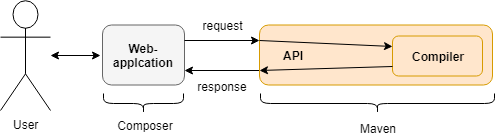
\includegraphics[scale=0.6]{images/maveninfra.png}
\caption{Current system infrastructure}
\label{fig:maveninfra}	
\end{figure}

Docker is designed to make it easier to create, deploy, and run applications by using \textit{\textbf{containers}}. A container can be thought of as a miniature, high-speed virtual machine. Prior to obtaining a container, we must first build an \textit{\textbf{image}}. To build an image we use a configuration file known as a  \textit{\textbf{Dockerfile}} in which one can specify commands that determine the environment of the image. These commands include downloading operating systems, setting file permissions, launching software, etc. After using a Dockerfile to build an image, we can then ``run'' it, which creates a corresponding live container, as illustrated in Figure \ref{fig:docker1}. It may be helpful to think of a container as an instance of an image. 

\begin{figure}[h]
\centering
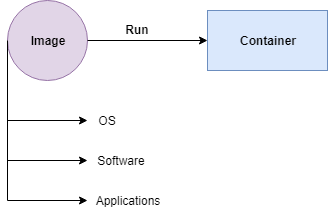
\includegraphics[scale=0.5]{images/docker1.png}
\caption{Creating a docker container from an image}
\label{fig:docker1}	
\end{figure}

The FunCompiler contains two Dockerfiles which are used to build two different images: one for the web-application, one for the compiler. Whilst we won't delve into specifics, these Dockerfiles contain the commands to retrieve dependencies (using Composer or Maven), execute builds and launch the servers. The exact contents of these Dockerfiles can be found in Appendices \ref{sec:web-dockerfile} and \ref{sec:compiler-dockerfile}

We can then use a sub-tool of Docker for running multi-container applications called Docker Compose. we use a YAML file named \textsf{docker-compose.yml} to define services. Each service generally corresponds to one image and thus one Dockerfile. In our case, we have two services, the web-application and the compiler. By invoking \texttt{docker-compose up}, we launch the services defined in \textsf{docker-compose.yml}, which entails automatically building the images from the Dockerfiles and then running these images, which creates the containers. Once both containers are live, the application is effectively up and running. To see the full contents of the FunCompiler's \textsf{docker-compose.yml} file refer to Appendix \ref{sec:docker-compose}.

There are a litany of advantages to using Docker but the fundamental point is that if another developer (or perhaps the system admin of a server deploying the application) was to obtain the source code of the FunCompiler, aslong as they had Docker installed, they could install every dependency, execute all builds and enable the entire FunCompiler application without having any of the constituent software available locally (e.g., PHP, Composer, Maven, Apache, etc.). Therefore, this makes the FunCompiler extremely portable because every machine, regardless of its own architecture, will build the application in precisely the same way, with precisely the same versions of all dependencies. 

With Docker implemented, we present the final system architecture of the FunCompiler, as demonstrated in Figure \ref{fig:finalinfra}. We see that both the web-application and the compiler are represented as containers and are both operating and communicating within a Docker environment.
\begin{figure}[h]
\centering
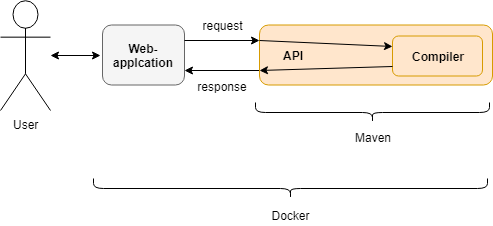
\includegraphics[scale=0.6]{images/finalinfra.png}
\caption{Final infrastructure of the FunCompiler}
\label{fig:finalinfra}	
\end{figure}

\chapter{Implementation}
In this chapter we give a high-level overview of the FunCompiler's implementation. As in Chapter 6, we decompose the FunCompiler into two separate components: the web-application and the compiler. 

Firstly, compiler. Secondly, web. Finally, tests

\section{Compiler Implementation}
In this section we discuss how we convert the original, stand-alone compiler into the micro-service as described in Chapter 6.  In order to accomplish this, two fundamental changes are necessary. Firstly, we must expose the compiler as an API in order to enable communication between itself and the web-application. Secondly, we must modify the implementation of the compiler to return a large amount of structured data pertaining to the compilation of a particular program. This information must be detailed enough that when sent as a response to the web-application, the web-application is equipped with enough data to build the animation of the compilation process.

\subsection{API}
Recall from Section \ref{sec:spark} that we intend to utilise a Java micro-framework known as Spark to encapsulate the compiler and create a compact API with a single endpoint. More specifically, the endpoint will be configured to accept HTTP POST requests. When the web-application desires to compile a Fun program as submitted by the user, it must make a POST request to the API  containing two query parameters: a program and a type. The value of program is simply the plain text version of the Fun program. The value of type corresponds to the button that was pressed as seen in Figure \ref{fig:code-editor-wireframe}, i.e., either contextual analysis or code generation. The following code snippet contains the complete implementation of this endpoint (the snippet also serves to support our previous claim that Spark allows us to create APIs in very few lines of code):
\begin{lstlisting}
post("/", (req, res) -> {
	res.type("application/json");
	String program = req.queryParams("program");
 	String type = req.queryParams("type");
	InputStream programInputStream = new ByteArrayInputStream(program.getBytes());
	return FunRun.execute(programInputStream, type);
}, gson::toJson);
\end{lstlisting} 

To clarify the exact functionality of this endpoint, we describe the purpose and effect of each line within the above code snippet:
\begin{description}
\item Line 1: We utilise Java 8 lambda expressions to define a POST route at the url ``/''. Within this expression we also declare the callback variables req and res, where req holds the contents of the request, and res will hold the contents of the response
\item Line 2: In order to provide structure to the data returned to the web-application, we state that the format of the response should be JSON.
\item Lines 3 and 4: Contained within the query parameters of the request is (as previously mentioned) the plain text of the input Fun program and selected compilation type. We extract these values from the parameters and store them in \texttt{String} variables.
\item Line 5: We now convert the input program, currently stored as a \texttt{String}, into an \texttt{InputStream}, which is the standard data type for input to ANTLR-based compilers.
\item Line 6: It is the \texttt{execute()} method defined within the FunRun module that is responsible for actually compiling the program. As arguments we supply the \texttt{InputStream} along with the compilation type. The return value of the \texttt{execute()} method is an object of the FunResponse class, which contains information collected during the compilation of the program. The data stored within this object is ultimately what the web-application uses to build the animation. The contents of the FunResponse class will be discussed in detail within the next section.
\item Line 7: In order to return a JSON response from the API as specified in line 2, we use a Java library named GSON which permits the conversion of Java objects (and the data contained within) to JSON objects.
\end{description}

\subsection{The FunResponse Object}
In order to build a data set containing various details relevant to the compilation of a program, we create a class named FunResponse. For each program that we intend to compile, we instantiate a new object of this class, which is returned upon completion of the compilation. It is within the instance variables of this class that we store the information regarding a program's compilation. The following code snippet shows the six instance variables (with access modifiers removed) that are declared within the FunResponse class:
\begin{lstlisting}
int numSyntaxErrors;
int numContextualErrors;
List<String> syntaxErrors;
List<String> contextualErrors;
JsonArray treeNodes;
JsonArray nodeOrder;
\end{lstlisting}

In the interest of brevity, we won't go into the details of how the values of these variables are derived or collected, however, we will consider the contents of each variable. In particular, we consider how to interpret the value of the variables \texttt{treeNodes} and \texttt{nodeOrder}, which store a representation of the AST alongside defining the order in which the animation should occur over the AST.

\subsubsection{Syntax \& Contextual Errors}
Lines 1 and 2 in the above code snippet simply collect the number of syntactic/contextual errors the compiler detects within the input program, whereas lines 3 and 4 collect a list of the actual error messages, including line and character number. In the case that there is no errors within the input program, these variables will remain empty, however, if errors are present the web-application can retrieve these values from the API response and report them to the user.

\subsubsection{AST Representation}
Within the \texttt{treeNodes} variable we store an array of nodes representing the input program's AST. Each node is represented by a JSON object that contains four fields of information:
\begin{itemize}
\item An ID, uniquely representing the node.
\item A parent ID, representing the parent of this node.
\item A node name, representing the type of the node (e.g, VAR, ID, PROC, etc.)
\item A node value, the text to be visually displayed within the web-applications' AST (in most cases, this is the same as the node name).
\end{itemize}
This array of nodes form a flat, hierarchical representation of an AST. For example, consider the following array of JSON objects:
\begin{lstlisting}
{
    "id": 306481855,
    "nodeName": "DIV",
    "nodeValue": "DIV",
    "parentId": 1670278882
},
{
    "id": 254315796,
    "nodeName": "ID",
    "nodeValue": "n",
    "parentId": 306481855
},
{
    "id": 532745069,
    "nodeName": "NUM",
    "nodeValue": "2",
    "parentId": 306481855
}
\end{lstlisting}
Within this example we can see that we have three different types of node, a \texttt{DIV}, an \texttt{ID} and a \texttt{NUM}. By examining the ``id'' of the \texttt{DIV} node and the ``parentId'' of the \texttt{ID} and \texttt{NUM} nodes, it is clear to see that \texttt{ID} and \texttt{NUM} are children of \texttt{DIV}. Therefore, we can use this knowledge to build the AST that is represented by this array, as illustrated in Figure \ref{fig:treeNodes}. The web-application will apply the same logic in order to take a much larger array of nodes and display the AST within the user interface.

 \begin{figure}[h]
\centering
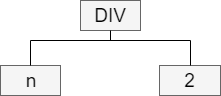
\includegraphics[scale=0.6]{images/treeNodes.png}
\caption{The AST represented by the above node array}
\label{fig:treeNodes}	
\end{figure}

\subsubsection{Animation Order \& Augmentations}
Like \texttt{treeNodes}, \texttt{nodeOrder} again contains an array of JSON objects representing nodes within the AST. However, the order of the nodes in \texttt{nodeOrder} correspond to the order in which they were visited during compilation, and thus the order they should be visited during the animation. Each node corresponds to exactly one node in the AST and the same node may appear multiple times. Along with dictating the order of the animation, each node with \texttt{nodeOrder} also contains all the augmentations that should be displayed with that node, this includes explanatory messages, type/address table information, code templates and object code. The type of augmentations that are stored within nodes are dependent upon the compiler type parameter we discussed in Section 7.1.1, for example, code templates and object are not included if the compilation type is contextual analysis. 

\begin{lstlisting}
"id": 2010337291,
"explanations": [
	"Walk expr1"
],
"table": [
	{
		"scope": "global",
		"id": "read",
		"type_address": "void -> int"
	},
	{
		"scope": "global",
		"id": "write",
		"type_address": "int -> void"
	},
	{
		"scope": "global",
		"id": "n",
		"type_address": "int"
	},
	{
		"scope": "local",
		"id": "main",
		"type_address": "void -> void"
	}
]
 \end{lstlisting}

%I Honestly reckon I can get away with just explaining the FunResponse and the contents of the fields - without going into inordindate details about the AST or CA or CG. This way I can go into more detail here about the specific contents of each field, and who cares about how they were actually gotten.
\section{Web-application}
\subsection{Animation}
\subsection{...}
\section{Testing?}
  
%Maybe say REST API but idk what that means atm.

%Put in implementation mayb
%Consequently, it was decided that the FunCompiler would follow the principles of single-page applications (SPAs). SPAs aim to significantly reduce the number of page refreshes websites undergo when the user requests new information or desires to see a different view (i.e., clicks a button). Treating the FunCompiler as an SPA would mean that when users, for example, submit a Fun program, the application will dynamically load the animation into view, without requiring a page refresh. The advantage of SPAs is that for small websites, you can create a much faster workflow which appears seamless. SPAs do have downsides, usually in terms of forcing too much processing on the client when websites grow large, and search engine optimisation. Fortunately, the FunCompiler suffers from neither of these problems.

%\subsection{Fun Specification}
%Since most users of the FunCompiler will be students enrolled in the Programming Languages course at Glasgow University, they will likely already have access to the full specification of the Fun language. However, embedding the Fun specification within the web application is valuable for two reasons. One, it is simply a matter of convenience, students will be able to find all the resources they need in one place. Two, inclusion of the specification helps not preclude the possibility that users could be non-students, as they would not have access to the specification otherwise. 

%For the purposes of this project we will be required to make significant alterations to the code base of the compiler. Included in the response that the compiler API returns to the web-application will be what is effectively a large set of metadata about the compilation. This metadata will be required to contain sufficient enough information that the web-application can construct a representation of the AST, allow animations over the AST, and display correctly timed augmentations alongside the animation.

%%%%%%%%%%%%%%%%
%              %
%  APPENDICES  %
%              %
%%%%%%%%%%%%%%%%
\begin{appendices}
\chapter{Configuration Files}
\section{pom.xml}
\label{sec:pom.xml}
\begin{lstlisting}
<?xml version="1.0" encoding="UTF-8"?>
<project xmlns="http://maven.apache.org/POM/4.0.0"
  xmlns:xsi="http://www.w3.org/2001/XMLSchema-instance"
  xsi:schemaLocation="http://maven.apache.org/POM/4.0.0
                      http://maven.apache.org/xsd/maven-4.0.0.xsd">
  <modelVersion>4.0.0</modelVersion>

  <groupId>api</groupId>
  <artifactId>api</artifactId>
  <version>1.0</version>

  <dependencies>
    <dependency>
      <groupId>com.sparkjava</groupId>
      <artifactId>spark-core</artifactId>
      <version>2.0.0</version>
    </dependency>
    <dependency>
      <groupId>org.slf4j</groupId>
      <artifactId>slf4j-simple</artifactId>
      <version>1.7.21</version>
    </dependency>
    <dependency>
      <groupId>org.antlr</groupId>
      <artifactId>antlr4-runtime</artifactId>
      <version>4.5.3</version>
    </dependency>
    <dependency>
      <groupId>com.google.code.gson</groupId>
      <artifactId>gson</artifactId>
      <version>2.8.0</version>
    </dependency>
  </dependencies>

  <build>
    <plugins>
      <plugin>
        <groupId>org.apache.maven.plugins</groupId>
        <artifactId>maven-jar-plugin</artifactId>
        <version>2.4</version>
        <configuration>
          <finalName>api</finalName>
          <archive>
            <manifest>
              <addClasspath>true</addClasspath>
              <mainClass>api.Api</mainClass>
              <classpathPrefix>dependency-jars/</classpathPrefix>
            </manifest>
          </archive>
        </configuration>
      </plugin>
      <plugin>
        <groupId>org.apache.maven.plugins</groupId>
        <artifactId>maven-compiler-plugin</artifactId>
        <version>3.1</version>
        <configuration>
          <source>1.8</source>
          <target>1.8</target>
        </configuration>
      </plugin>
      <plugin>
        <groupId>org.apache.maven.plugins</groupId>
        <artifactId>maven-assembly-plugin</artifactId>
        <executions>
          <execution>
            <goals>
              <goal>attached</goal>
            </goals>
            <phase>package</phase>
            <configuration>
              <finalName>api</finalName>
              <descriptorRefs>
                <descriptorRef>jar-with-dependencies</descriptorRef>
              </descriptorRefs>
              <archive>
                <manifest>
                  <mainClass>api.Api</mainClass>
                </manifest>
              </archive>
            </configuration>
          </execution>
        </executions>
      </plugin>
      <plugin>
        <groupId>org.antlr</groupId>
        <artifactId>antlr4-maven-plugin</artifactId>
        <version>4.5.3</version>
        <executions>
          <execution>
            <goals>
              <goal>antlr4</goal>
            </goals>
            <configuration>
              <sourceDirectory>${basedir}/src/main/antlr4/api</sourceDirectory>
              <listener>false</listener>
              <visitor>true</visitor>
            </configuration>
          </execution>
        </executions>
      </plugin>
    </plugins>
  </build>

</project>
\end{lstlisting}

\section{Web-Application Dockerfile}
\label{sec:web-dockerfile}
\begin{lstlisting}
# Use a PHP7.0 image that is packaged with the Apache web server
FROM php:7.0-apache
# Download composer and install composer.phar in /usr/local/bin
RUN curl -sS https://getcomposer.org/installer | php -- --install-dir=/usr/local/bin --filename=composer
# Create the 'app' directory and set to be the working directory of the container
WORKDIR /app
# Copy all files in current directory to the working directory of the container
COPY . /app
# Update packages and install composer and PHP dependencies.
RUN apt-get update -yqq
RUN apt-get install git zlib1g-dev -yqq
RUN pecl install xdebug
# Compile PHP, include these extensions.
RUN docker-php-ext-install zip
RUN docker-php-ext-enable xdebug
# Use the 'composer.json' file to download any PHP dependencies (including Laravel)
RUN composer install
RUN cp .env.example .env
RUN php artisan key:generate
\end{lstlisting}

\section{Compiler Dockerfile}
\label{sec:compiler-dockerfile}
\begin{lstlisting}
# Use an OpenJDK8 image to run and compile Java files
FROM openjdk:8
# Install Maven in the container
RUN apt-get update
RUN apt-get install -y maven
# Create the 'compiler' directory and set to be the working directory of the container
WORKDIR /compiler
# Add 'pom.xml' to the container
ADD pom.xml /compiler/pom.xml
# Download maven dependencies (e.g., Antlr and Spark)
RUN ["mvn", "dependency:resolve"]
RUN ["mvn", "verify"]
# Add the source directory
ADD src /compiler/src
# Compile and package into a fat jar
RUN ["mvn", "package"]
\end{lstlisting}

\section{docker-compose.production.yml}
\label{sec:docker-compose}
\begin{lstlisting}
# Version of the docker-compose file format
version: '3'

# Individual components of the overall product (the web app and the compiler api)
services:
    compiler:
        # Name the resulting container
        container_name: FunCompiler
        # Configuration options applied at build time (i.e., location of Dockerfile)
        build: ./compiler
        # Launch the Spark web server (the compiler API)
        command: java -jar target/api-jar-with-dependencies.jar
        # Expose port 8001 on the host and 4567 on the container
        ports:
            - 8001:4567

    app:
        # Name the resulting container
        container_name: FunApp
        # Configuration options applied at build time (i.e., location of Dockerfile)
        build: ./app
        # Launch the Laravel server (the web app)
        command: php artisan serve --host=0.0.0.0 --port=8000
        # Expose port 8000 on the host and port 8000 on the container
        ports:
            - 8000:8000
        # Starts services in dependency order, i.e., compiler before app
        depends_on:
            - compiler
\end{lstlisting}

\end{appendices}

%%%%%%%%%%%%%%%%%%%%
%   BIBLIOGRAPHY   %
%%%%%%%%%%%%%%%%%%%%

\bibliographystyle{plain}
\bibliography{bib}

\end{document}
